\chapter{Návrh architektury}\label{chap:architecture}

\begin{chapterabstract}
	Kapitola popisuje celkovou architekturu systému, návrh jednotlivých komponent a~datový model. Nejprve je představen přehled systému a~komunikace mezi jeho částmi, následně je podrobně popsána architektura backendu, frontendu a~mobilní aplikace.
\end{chapterabstract}

\section{Přehled systému}

Systém se skládá ze tří hlavních komponent, které spolu komunikují prostřednictvím REST API přes protokol HTTPS (viz obrázek~\ref{fig:system-architecture}):

\begin{itemize}
	\item \textbf{Backend} -- serverová aplikace (Spring Boot) poskytující REST API, business logiku, generování exportů a~přístup k~databázi PostgreSQL. Backend je nasazen na linuxovém VPS serveru za reverse proxy Nginx.
	\item \textbf{Frontend} -- jednostránková webová aplikace (React) pro správu majetku, uživatelů a~vyhodnocení inventury. Komunikuje výhradně s~backendem prostřednictvím REST API.
	\item \textbf{Mobilní aplikace} -- nativní Android aplikace pro inventuru v~terénu. Disponuje vlastní lokální databází (Room/SQLite) pro offline režim a~se serverem se synchronizuje na vyžádání.
\end{itemize}

\begin{figure}[H]\centering
	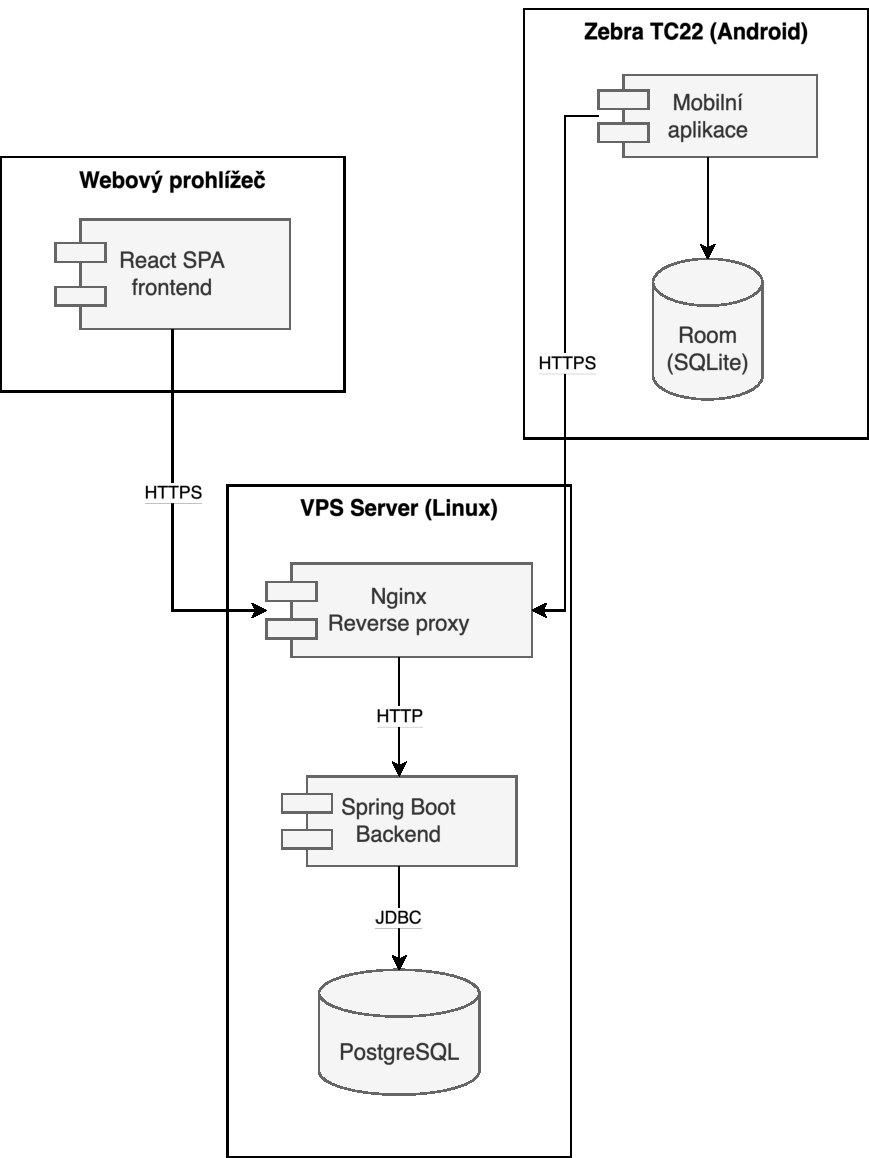
\includegraphics[width=0.85\textwidth]{images/system-architecture.pdf}
	\caption{Diagram architektury systému}\label{fig:system-architecture}
\end{figure}

Frontend ani mobilní aplikace spolu přímo nekomunikují -- veškerá výměna dat probíhá prostřednictvím backendu. Tento přístup centralizuje business logiku a~zjednodušuje bezpečnostní model, neboť autentizace a~autorizace jsou řešeny na jednom místě.

\section{Architektura backendu}\label{sec:backend-arch}

Backend je organizován jako modulární monolitická aplikace -- každá doménová oblast (karty majetku, autentizace, číselníky, inventurní audit, přílohy) má vlastní balíček obsahující celý vertikální řez od kontroleru po repozitář. Tento přístup byl zvolen oproti klasickému vrstvovému uspořádání (všechny kontrolery v~jednom balíčku, všechny služby v~druhém), protože drží související kód pohromadě a~usnadňuje orientaci v~projektu -- při práci na konkrétní funkčnosti není nutné přecházet mezi vzdálenými částmi stromu zdrojových souborů.

\subsection{Vrstvená architektura}

Každý modul dodržuje konzistentní třívrstvý vzor odpovídající klasické enterprise architektuře~\cite{fowler-eaa}:

\begin{enumerate}
	\item \textbf{Controller} (\texttt{@RestController}) -- přijímá HTTP požadavky, provádí vstupní validaci prostřednictvím anotace \texttt{@Valid} a~deleguje zpracování na service vrstvu. Vrací \texttt{ResponseEntity} s~příslušným HTTP kódem.
	\item \textbf{Service} -- definovaný jako rozhraní (\texttt{IXxxService}) s~implementací v~podbalíčku \texttt{implementation}. Oddělení rozhraní od implementace je běžný vzor ve Spring ekosystému -- dodržuje SOLID princip Dependency Inversion, usnadňuje mockování v~unit testech a~zjednodušuje případné rozšíření o~alternativní implementaci. Service obsahuje business logiku a~řídí transakce prostřednictvím anotace \texttt{@Transactional}.
	\item \textbf{Repository} -- rozhraní rozšiřující \texttt{JpaRepository}, které poskytuje přístup k~databázi. Dotazy jsou buď odvozeny z~názvu metody, nebo definovány explicitně anotací \texttt{@Query}.
\end{enumerate}

Mezi vrstvami je zajištěna separace dat prostřednictvím vzoru DTO (Data Transfer Object)~\cite{fowler-eaa}. Mapování mezi entitami a~DTO zajišťuje knihovna MapStruct, která generuje mapovací kód v~době kompilace. Kontrolery nikdy nepracují přímo s~JPA entitami -- vždy přijímají a~vracejí DTO objekty.

\subsection{Modulární struktura}

Backend je rozdělen do následujících modulů:

\begin{itemize}
	\item \textbf{auth} -- autentizace, správa uživatelů, bezpečnostní konfigurace (JWT filtry, Spring Security)
	\item \textbf{card} -- CRUD operace nad kartami majetku, filtrování, generování exportů (PDF, Excel, ZPL)
	\item \textbf{attachment} -- správa souborových příloh ke~kartám majetku
	\item \textbf{inventoryaudit} -- import inventurních dat z~mobilní aplikace, výpočet rozdílů, projekce změn
	\item \textbf{dictionary} -- pět číselníkových podmodulů (umístění, skupiny, třídy, způsoby pořízení, způsoby vyřazení), každý se shodnou strukturou
	\item \textbf{entity} -- centralizované JPA entity sdílené napříč moduly
	\item \textbf{exception} -- globální zpracování výjimek (\texttt{@RestControllerAdvice}). Doménové výjimky jsou převedeny na strukturované JSON odpovědi s~příslušným HTTP kódem. Na frontendu jsou chyby zobrazeny toast notifikacemi, v~mobilní aplikaci barevně odlišenými stavovými zprávami.
	\item \textbf{config} -- konfigurace aplikace (OpenAPI dokumentace, kódování hesel)
\end{itemize}

Struktura balíčků je znázorněna na obrázku~\ref{fig:package-backend}. Všechny doménové moduly závisí na balíčku \texttt{entity}, který obsahuje sdílené JPA entity.

\begin{figure}[H]\centering
	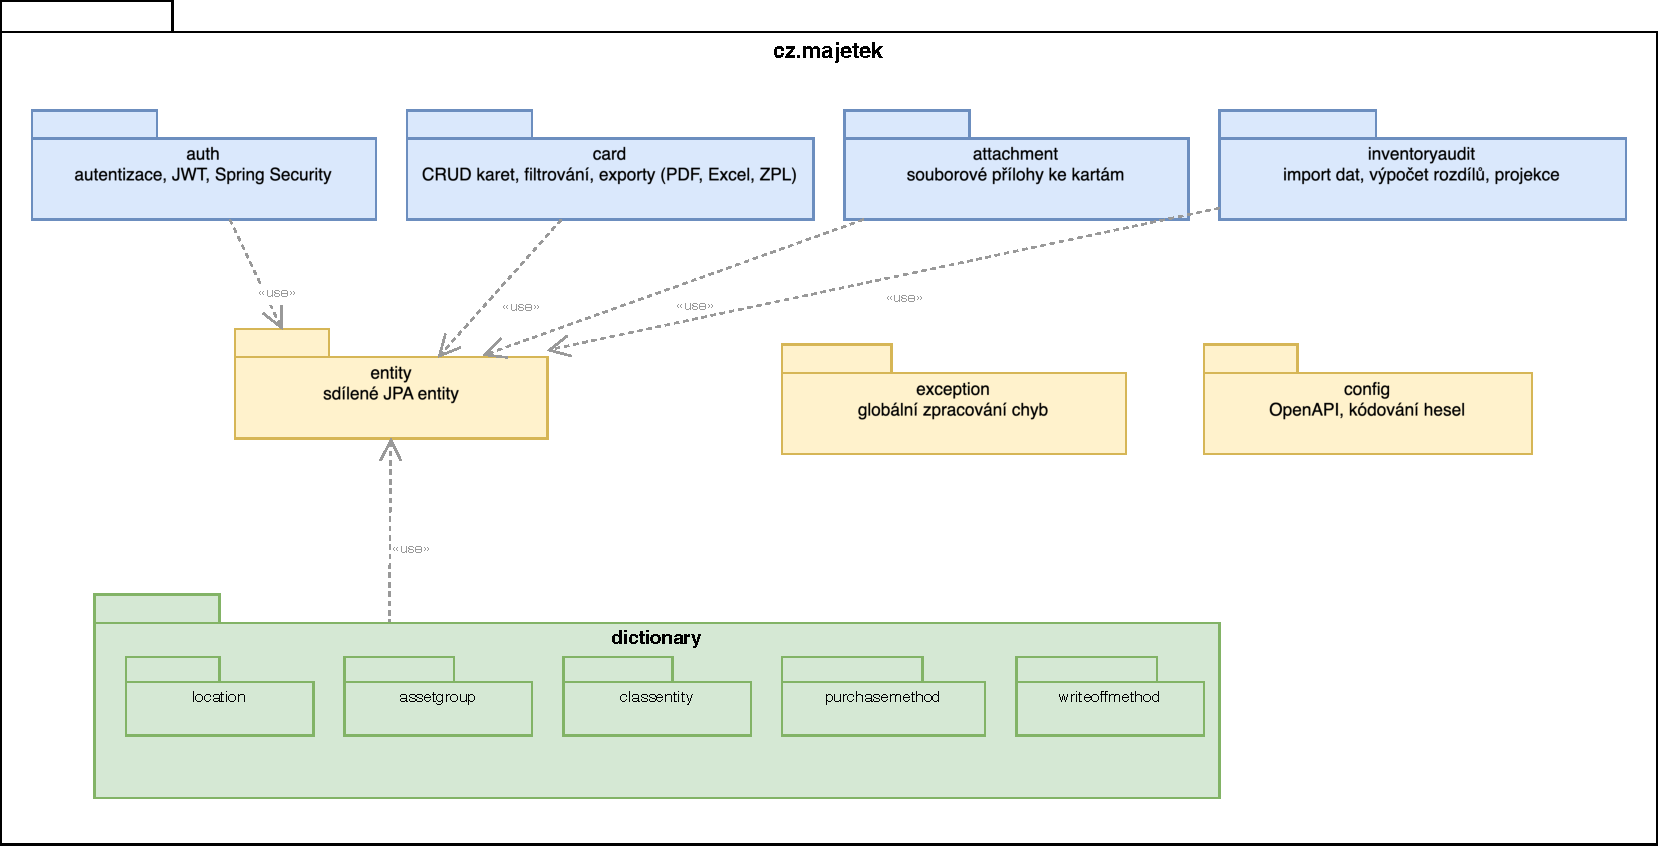
\includegraphics[width=\textwidth]{images/package-backend.pdf}
	\caption{Diagram balíčků backendu}\label{fig:package-backend}
\end{figure}

\subsection{Bezpečnostní model}

Autentizace je realizována pomocí JSON Web Tokenů (JWT)~\cite{jwt}. Systém využívá dvě samostatné bezpečnostní filter chains v~rámci Spring Security:

\begin{enumerate}
	\item \textbf{Basic Auth chain} -- zachytává výhradně požadavek na přihlášení (\texttt{POST /api/auth/login}). Po ověření přihlašovacích údajů vygeneruje access token (krátká platnost) a~refresh token (delší platnost).
	\item \textbf{JWT Bearer chain} -- zachytává všechny ostatní API požadavky. Filtr \texttt{JwtAuthenticationFilter} extrahuje token z~hlavičky \texttt{Authorization: Bearer}, ověří jeho platnost a~nastaví bezpečnostní kontext.
\end{enumerate}

Access token je přenášen v~HTTP hlavičce, refresh token výhradně v~\texttt{httpOnly} cookie s~příznakem \texttt{Secure} a~\texttt{SameSite=Strict}. Při obnovení (endpoint \texttt{/api/\allowbreak auth/\allowbreak refresh}) server ověří platnost refresh tokenu, zkontroluje jeho jedinečný identifikátor (\texttt{jti}) oproti hodnotě uložené v~databázi a~vygeneruje nový pár tokenů. Starý refresh token je tímto invalidován -- jedná se o~tzv.\ rotaci tokenů, která prodlužuje session při aktivním používání a~zároveň zajišťuje, že kompromitovaný token nelze opakovaně použít. Celý autentizační tok je znázorněn na obrázku~\ref{fig:jwt-auth-flow}.

\begin{figure}[H]\centering
	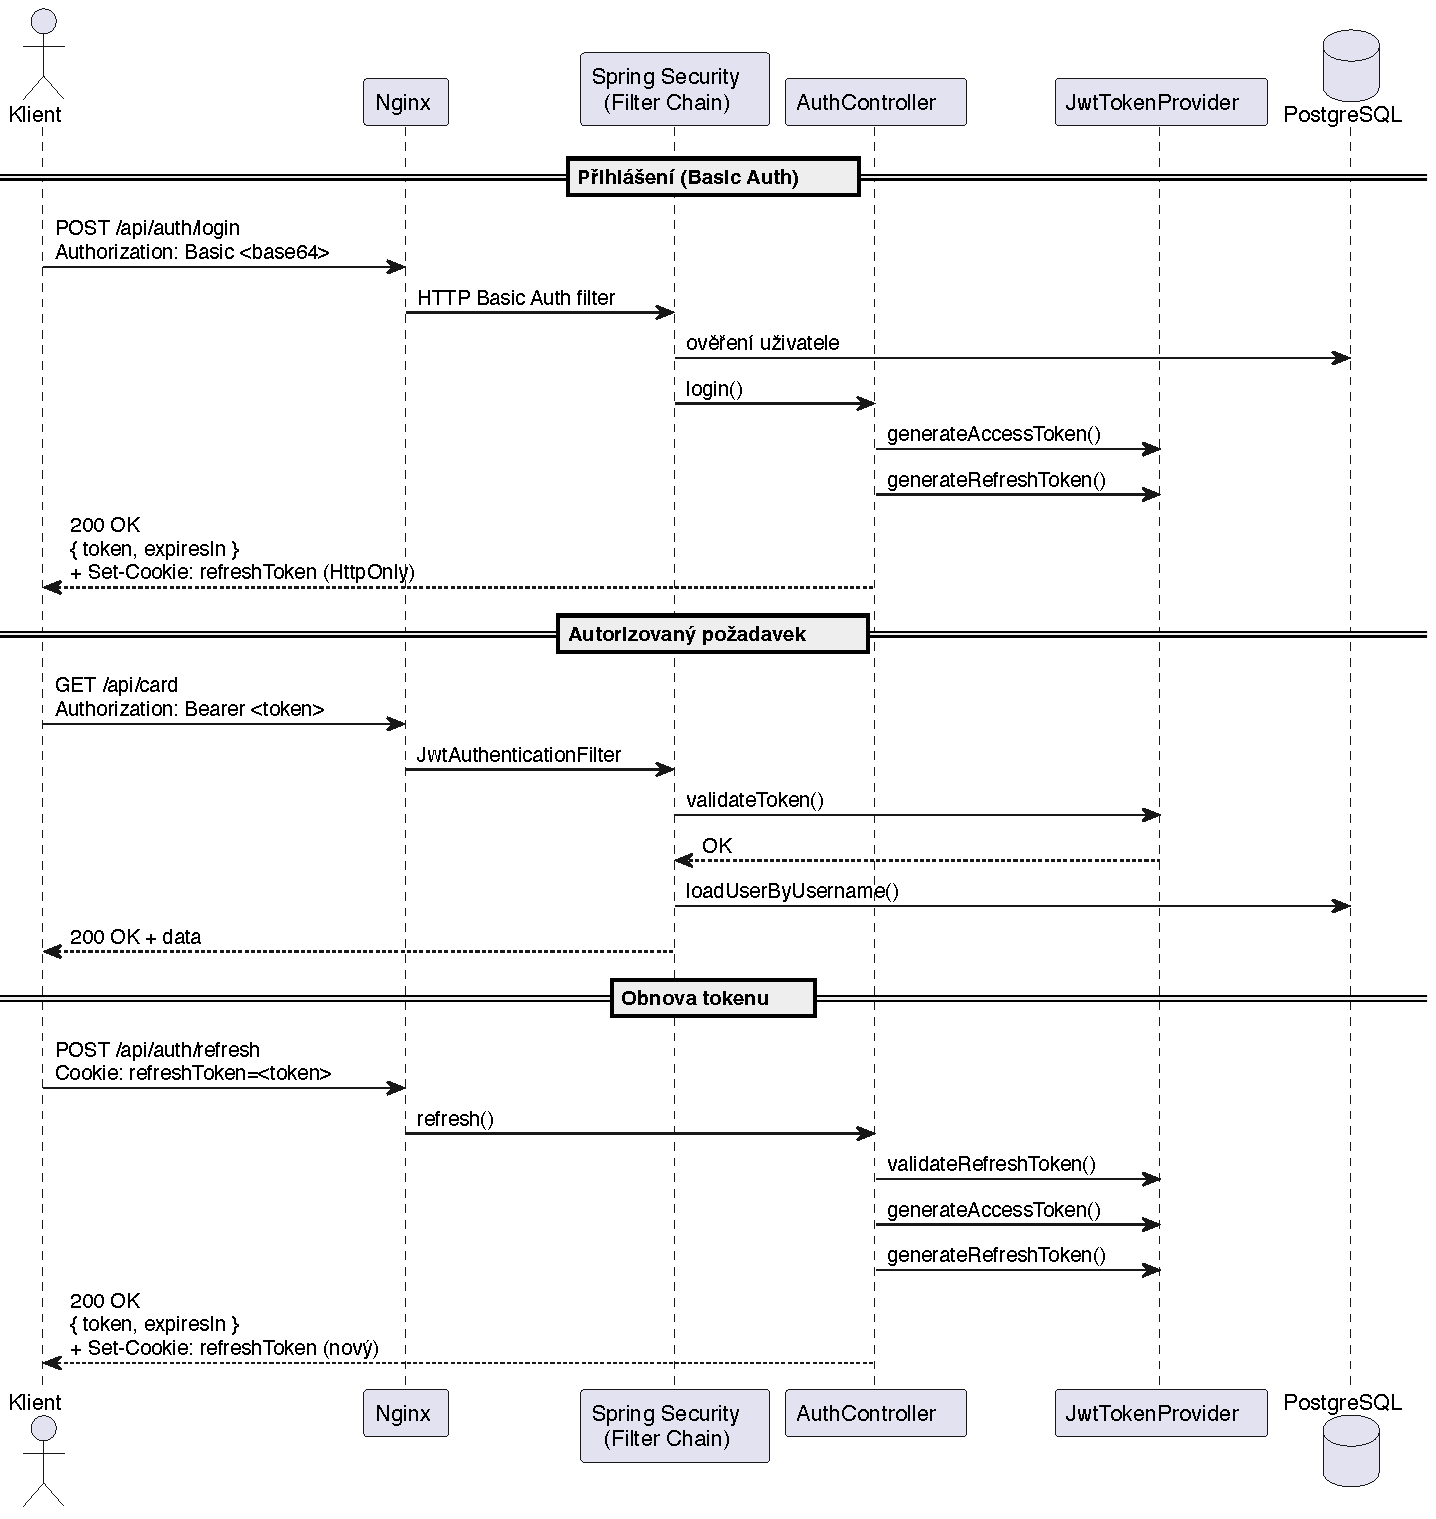
\includegraphics[width=\textwidth]{images/jwt-auth-flow.pdf}
	\caption{Sekvenční diagram autentizačního flow}\label{fig:jwt-auth-flow}
\end{figure}

Autorizace rozlišuje dvě role: \texttt{USER} a~\texttt{ADMIN}. Jediným endpointem omezeným na roli administrátora je registrace nového uživatele, chráněná anotací \texttt{@PreAuthorize}. Ostatní endpointy vyžadují pouze platný JWT token bez ohledu na roli.

\section{Architektura frontendu}

Frontend je jednostránková aplikace (SPA) v~Reactu a~TypeScriptu. Architektura je navržena s~důrazem na oddělení zodpovědností.

\subsection{Vrstvená architektura}

\begin{enumerate}
	\item \textbf{Services} (\texttt{services/}) -- čisté asynchronní funkce pro komunikaci s~API prostřednictvím knihovny Axios. Každá doménová entita má vlastní service soubor. Funkce transformují data z~API formátu do TypeScriptových typů.
	\item \textbf{Query hooks} (\texttt{hooks/queries/}) -- wrappery nad TanStack Query, které zapouzdřují volání service funkcí. Query hooky zajišťují cachování, automatickou invalidaci a~správu serverového stavu.
	\item \textbf{Komponenty} (\texttt{components/}) -- znovupoužitelné UI komponenty organizované podle domény (card, dictionary, report, inventoryAudit).
	\item \textbf{Stránky} (\texttt{pages/}) -- komponenty na úrovni route, které skládají jednotlivé UI komponenty do celých obrazovek.
\end{enumerate}

\subsection{Správa stavu}

Webová aplikace pracuje se dvěma kategoricky odlišnými typy stavu, které vyžadují odlišné řešení. \textbf{Serverový stav} odpovídá datům uloženým v~databázi (karty majetku, číselníky, inventurní záznamy) -- aplikace si jeho aktuální podobu pouze cachuje a~musí řešit zastarávání cache, opětovné načtení po~mutaci a~konzistenci napříč obrazovkami. \textbf{Klientský stav} se naopak týká informací existujících pouze v~prohlížeči (přihlášený uživatel, otevřená modalní okna, lokální UI volby) a~vyžaduje synchronizaci pouze v~rámci jedné aplikační instance.

Vzhledem k~odlišné povaze obou typů stavu byly zvoleny dvě specializované knihovny:

\begin{itemize}
	\item \textbf{Serverový stav} je spravován knihovnou TanStack Query. Veškerá data z~API jsou cachována s~dobou platnosti dvě minuty. Mutace po úspěchu buď invalidují příslušné cache klíče (plný refetch), nebo optimisticky aktualizují cache přímo.
	\item \textbf{Klientský stav} je omezen na autentizační údaje (přihlášený uživatel, JWT token, expirace) a~spravuje jej jediný Zustand store. Axios interceptor automaticky obnovuje vypršelý token prostřednictvím refresh endpointu před odesláním požadavku.
\end{itemize}

Všechny chráněné stránky jsou obaleny komponentou \texttt{PrivateRoute}, která ověřuje přítomnost platného JWT tokenu v~Zustand store a~nepřihlášeného uživatele přesměruje na přihlašovací stránku. Chráněné stránky jsou načítány líně (\texttt{React.lazy}) -- jejich kód se stáhne až při prvním přístupu, což zkracuje počáteční dobu načtení.

\subsection{Generický vzor pro číselníky}

Pět číselníkových stránek sdílí generickou komponentu \texttt{DictionaryPage<T>}, parametrizovanou typem entity. Komponenta přijímá hooky pro query a~mutace jako vlastnosti a~vykresluje tabulku s~operacemi vytvoření, přejmenování a~smazání. Konkrétní stránky (např.\ \texttt{LocationPage}) jsou pouze wrappery, které předávají příslušné hooky a~volitelné rozšíření (např.\ tlačítko tisku etikety u~lokací).

\section{Architektura mobilní aplikace}\label{sec:mobile-arch}

Mobilní aplikace je navržena jako jednoduchá nativní Android aplikace s~jednou Activity a~třemi fragmenty. Architektura je přizpůsobena specifickým požadavkům -- offline režim, vstup z~hardwarového skeneru a~provoz na enterprise zařízení Zebra TC22.

\subsection{Struktura uživatelského rozhraní}

Aplikace využívá jednu \texttt{MainActivity}, která hostuje tři fragmenty přepínané prostřednictvím spodní navigační lišty (\texttt{BottomNavigationView}):

\begin{enumerate}
	\item \textbf{ControlScanFragment} -- kontrolní snímání. Umožňuje naskenovat kód majetku a~zobrazit jeho detail bez zápisu do inventury. Slouží pro rychlé ověření identity položky.
	\item \textbf{InventoryScanFragment} -- inventurní snímání. Dvoustupňový proces: nejprve se naskenuje kód místnosti (nastavení aktuálního umístění), poté se postupně skenují kódy majetku. Každé naskenování vytvoří záznam v~lokální databázi.
	\item \textbf{DataTransferFragment} -- přenos dat. Umožňuje stáhnout aktuální data ze~serveru, nahrát inventurní záznamy zpět a~konfigurovat URL serveru.
\end{enumerate}

\subsection{Offline režim a~synchronizace}

Mobilní aplikace využívá knihovnu Room jako abstrakci nad SQLite. Lokální databáze obsahuje tři tabulky: \texttt{card} (karty majetku), \texttt{location} (lokace) a~\texttt{inventory\_audit} (inventurní záznamy). Data karet a~lokací jsou stažena ze~serveru před zahájením inventury; inventurní záznamy vznikají lokálně při skenování. Tabulka \texttt{inventory\_audit} má primární klíč \texttt{card\_id} -- každá karta může mít nejvýše jeden inventurní záznam. Opakované naskenování téže karty aktualizuje existující záznam (strategie \texttt{REPLACE}).

Synchronizace probíhá výhradně na explicitní pokyn uživatele:

\begin{itemize}
	\item \textbf{Stažení dat} -- aplikace ověří připojení k~síti, autentizuje se prostřednictvím Basic Auth, stáhne aktuální karty a~lokace a~atomicky je uloží do lokální databáze v~rámci jedné transakce.
	\item \textbf{Odeslání inventury} -- aplikace načte všechny lokální inventurní záznamy, serializuje je do formátu JSON a~odešle hromadným požadavkem na server (\texttt{POST /api/inventory-audit/insert-many}).
\end{itemize}

Stažení nových dat je zablokováno, pokud v~lokální databázi existují neodeslaná inventurní data -- tím je zabráněno nechtěné ztrátě práce. Autentizační tokeny i~přihlašovací údaje jsou uloženy v~šifrovaném úložišti \texttt{EncryptedSharedPreferences} (AES-256-GCM). Síťová konfigurace zakazuje nešifrovanou komunikaci (\texttt{cleartext traffic}). Celý protokol synchronizace mezi mobilní aplikací, lokální Room databází a~serverem znázorňuje obrázek~\ref{fig:sequence-sync}.

\begin{figure}[H]\centering
	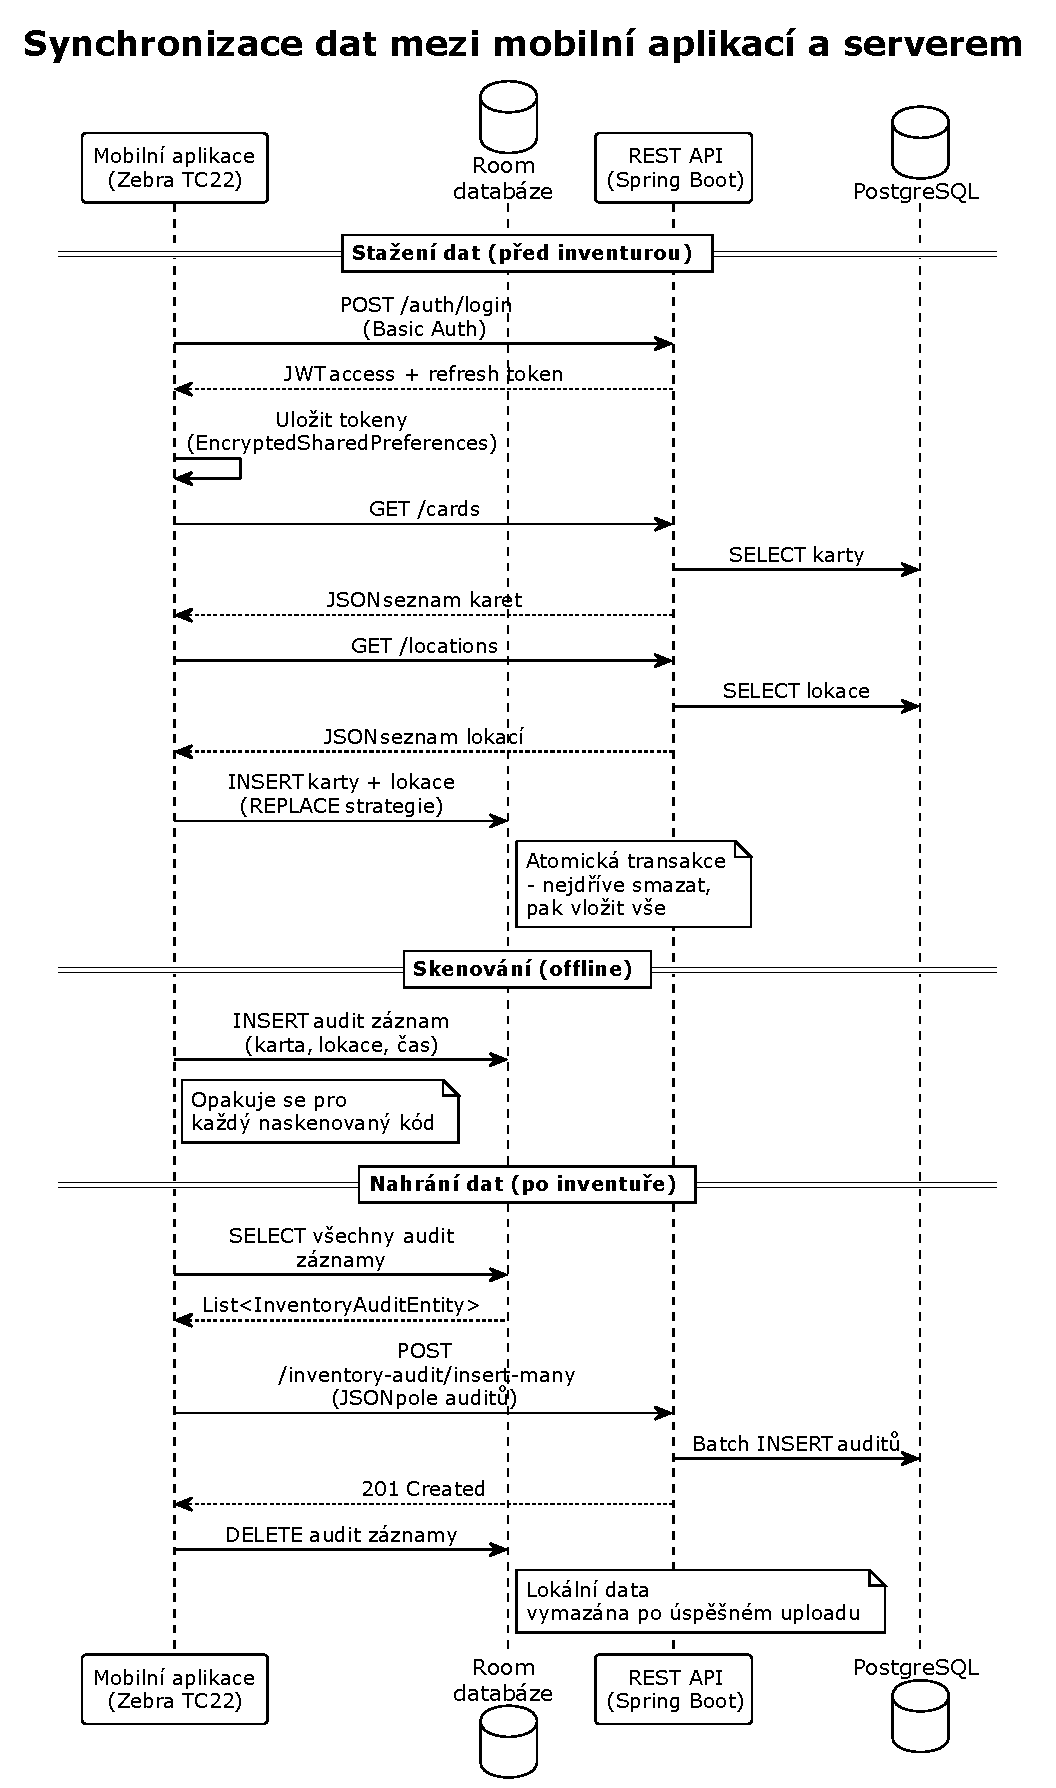
\includegraphics[width=\textwidth]{images/sequence-sync.pdf}
	\caption{Sekvenční diagram synchronizace dat mezi mobilní aplikací a~serverem}\label{fig:sequence-sync}
\end{figure}

\section{Datový model}

Datový model systému tvoří devět tabulek v~relační databázi PostgreSQL (viz obrázek~\ref{fig:er-diagram}). Centrální entitou je tabulka \texttt{card} (majetková karta), na~kterou se váží číselníkové tabulky, přílohy a~inventurní záznamy.

\begin{figure}[H]\centering
	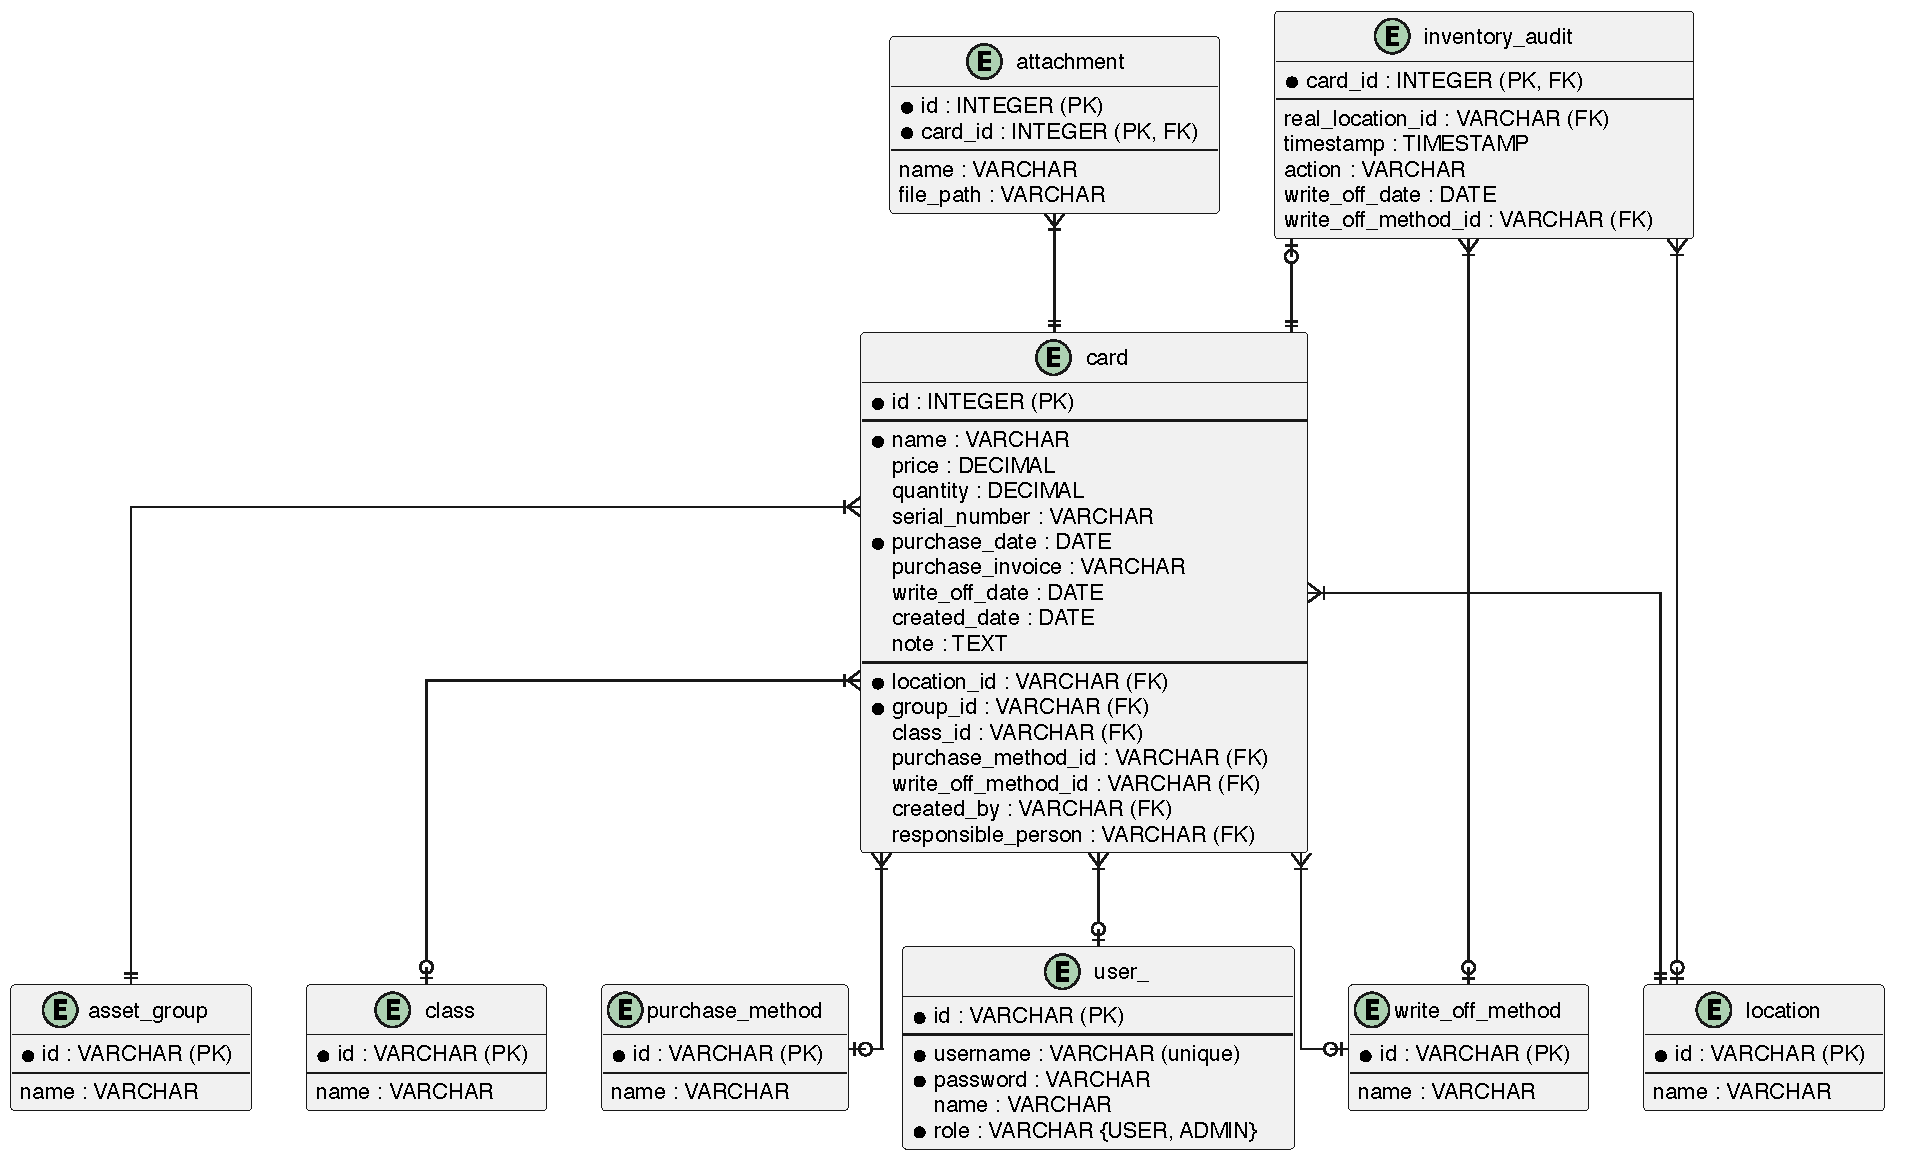
\includegraphics[width=\textwidth]{images/er-diagram.pdf}
	\caption{ER diagram datového modelu}\label{fig:er-diagram}
\end{figure}

\subsection{Popis entit}

\textbf{Card} (majetková karta) je hlavní entita systému. Identifikátor karty je celočíselný, přiřazovaný aplikační logikou. Toto číslo se tiskne na etiketu a~slouží jako inventární číslo v~účetní evidenci. Karta dále obsahuje název, cenu, množství, sériové číslo, datum pořízení, fakturu, poznámku a~vazby na číselníkové entity (umístění, třída, skupina, způsob pořízení, způsob vyřazení) a~uživatele (kdo kartu vytvořil, zodpovědná osoba).

\textbf{Číselníkové entity} (Location, AssetGroup, ClassEntity, PurchaseMethod, WriteOffMethod) sdílejí shodnou strukturu -- textový identifikátor (primární klíč) a~název. Použití přirozeného klíče (natural key) místo umělého auto-increment identifikátoru je záměrné a~inspirováno přístupem ERP systémů -- kódy zadává uživatel ručně (např.\ číslo místnosti, zkratka skupiny) a~v~celém systému se s~nimi pracuje přímo, bez nutnosti překladu přes umělé ID. Číselníkové entity definují přípustné hodnoty pro atributy majetkových karet.

\textbf{Attachment} (příloha) umožňuje připojit soubory ke~kartě majetku. Využívá kompozitní primární klíč složený z~identifikátoru přílohy a~identifikátoru karty.

\textbf{InventoryAudit} (inventurní záznam) uchovává výsledek inventury pro jednu kartu -- skutečné umístění, časové razítko naskenování a~po vyhodnocení i~zvolenou akci (ponechat umístění, změnit umístění, vyřadit). Primární klíč je sdílen s~kartou (\texttt{@MapsId}) -- každá karta může mít nejvýše jeden inventurní záznam.

\textbf{User} (uživatel) obsahuje přihlašovací údaje a~roli (\texttt{USER} nebo \texttt{ADMIN}). Tabulka je v~databázi pojmenována \texttt{user\_} s~podtržítkem, protože \texttt{user} je rezervované slovo v~PostgreSQL. Uživatel je volitelně referencován z~karty jako tvůrce záznamu nebo zodpovědná osoba.


